\documentclass[handout,sanserif,mathserif]{beamer}

%% packages
%\usepackage{times}
\usepackage{graphicx}
\usepackage{fancyheadings}
\usepackage{epsfig}
\usepackage{colordvi}
\usepackage{color}
\usepackage{amssymb}
\usepackage{amsmath}
\usepackage{verbatim}
\usepackage{theorem}
\usepackage{graphics}
\usepackage{float}
\usepackage{psfrag}
\usepackage{rotating}
\usepackage{bm}

%% macros
\newcommand{\myskip}{\vskip 0.125in}

%% settings
\definecolor{Orange}{rgb}{1,0.5,0}
\definecolor{RoyalBlue}{RGB}{65,105,225}

\setbeamertemplate{frametitle}[default][center]
\setbeamertemplate{itemize item}[square]
\setbeamertemplate{itemize subitem}[circle]

\setbeamercolor{frametitle}{fg=RoyalBlue}
\setbeamercolor{itemize item}{fg=black}
\setbeamercolor{itemize subitem}{fg=black}

\begin{document}

\begin{frame}
\frametitle{Basic Tenets of Zipf's Law}

\begin{itemize}
\item Words are not even distributed
\begin{itemize}
\item 10\% of words in text documents are made of ``the'' and ``of''
\end{itemize}
\end{itemize}

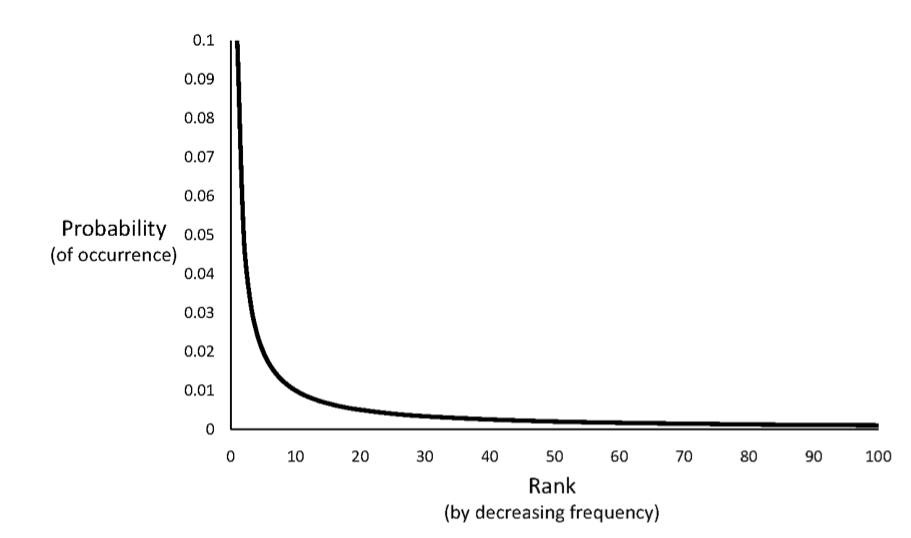
\includegraphics[height=1.5in]{zipf-1.png}

\begin{itemize}
\item Zipf's Law describes the relationship between ranking (importance) and frequency
\begin{itemize}
\item The rank ($r$) of a word times its frequency ($f$) is approximately a constant($k$)  $\longrightarrow$  $k \approx r f $ 
\item The probability of a word's occurrence times its rank is approximately a constant ($c$)  $\longrightarrow$ $c \approx r P$ [for English $c \approx 0.1$]
\end{itemize}
\end{itemize}
\end{frame}


\begin{frame}
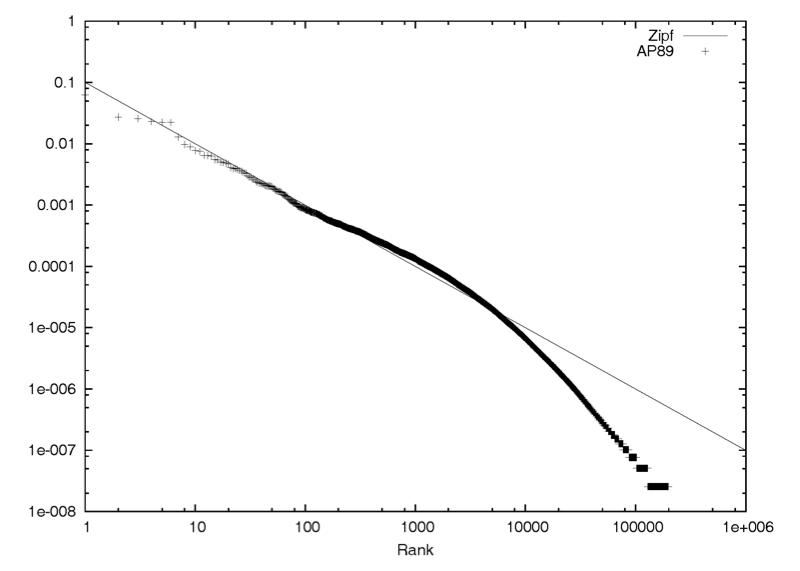
\includegraphics[height=2.0in]{zipf-2.png}

On a log-log plot of actual data agains the theoretical Zipf's Law plot, we observe that data falls apart for lower frequency (higher rank) words. Since $P = c/r$ and by taking the log of both sides we now have: $\log(P) = \log(c) - \log(r)$.  If $c$ is a constant then the slope of the line is $-\log(r)$.

\end{frame}

\begin{frame}
\frametitle{Proportion of Words}

What is the proportion of words with a given frequency?  If you have the words frequency (usually derive from a small sample), can you calculate the ratio of the word to the collection?

\begin{itemize}

\item Words occurring $n$ times has rank $r = k/n$
\item Number of words with frequency $n$ is
$$ r_{n} - r_{n+1} = \frac{k}{n} - \frac{k}{n+1} = \frac{k}{n(n+1)} $$
\item Proportion (ratio) found by dividing by the total number of words
\item Proportion with frequency $n$ is $1/(n(n+1))$
\end{itemize}

\end{frame}


\begin{frame}
\frametitle{Page rank {\bf without} a random jump factor $\lambda$}

If $v$ is a webpage in the set $B_u$ where 

\begin{itemize}
\item $v$ contains at least one link to page $u$
\item $L_v$ are the number of links from page $v$
\end{itemize}

Then formula for calculating page rank for $u$  is:

$$ 
  Pr(u) = \sum_{v\in B_u} { \frac{PR(v)}{L_v} }
$$

In other words, the rank of page $u$ is the sum of the rank each page $v$ divided by the number of its outgoing links.  $L_v$ are, of course, free of duplicates.

\end{frame}

\begin{frame}

Let's assume that our document collection is as followed:

\begin{itemize}

\item Document A has links to documents B and C
\item Document B has a link to document C but not document A and therefore does not contribute to A's ranking
\item Document C has a link to document A but not to document B and therefore does not contribute B's ranking

\end{itemize}

Let's calculate the ranking in $k$ iterations.  For the first iteration, we assume all pages have equal rank $\approx 0.33$.  Then using results from this step to calculate the next iteration.  Repeat until convergence.

\vskip 0.125 in

\end{frame}

\begin{frame}

{\color{RoyalBlue}{\Large First iteration}}

\vskip 0.125 in

Calculate page rank for $A$.  Because $B$ does not link to $A$ so we do not consider it:
$$
PR(A) = \frac{PR(C)}{1} = \frac{0.33}{1} = 0.33
$$

Calculate page rank for $B$.  Because $C$ does not link to $B$ so we do not consider it:
$$
PR(B) = \frac{PR(A)}{2} = \frac{0.33}{2} \approx 0.17
$$

Calculate page rank for $C$:
$$ 
PR(C) = \frac{PR(A)}{2} + \frac{PR(B)}{1} = \frac{0.33}{2} + \frac{0.33}{1} \approx 0.50
$$

\end{frame}

\begin{frame}

{\color{RoyalBlue}{\Large Second iteration}}
\vskip 0.125 in

Substitute the above results for $PR(A)$, $PR(B)$, and $PR(C)$:

$$
PR(A) = \frac{PR(C)}{1} = \frac{0.50}{1} = 0.50
$$

$$
PR(B) = \frac{PR(A)}{2} = \frac{0.33}{2} \approx 0.17
$$

$$ 
PR(C) = \frac{PR(A)}{2} + \frac{PR(B)}{1} = \frac{0.33}{2} + \frac{0.17}{1} \approx 0.33
$$

\end{frame}

\begin{frame}

{\color{RoyalBlue}{\Large Third iteration}}
\vskip 0.125 in

Substitute the above results for $PR(A)$, $PR(B)$, and $PR(C)$:

$$
PR(A) = \frac{PR(C)}{1} = \frac{0.33}{1} = 0.33
$$

$$
PR(B) = \frac{PR(A)}{2} = \frac{0.50}{2} = 0.25
$$

$$ 
PR(C) = \frac{PR(A)}{2} + \frac{PR(B)}{1} = \frac{0.50}{2} + \frac{0.17}{1} \approx 0.42
$$

Continue these steps until the numbers converge.  In other words, the next iteration no longer updates the $PR$ values or the updated values are less than some small value $\epsilon$

\end{frame}

\begin{frame}
\frametitle{Page rank {\bf with} a random jump factor $\lambda$}

If we take random page jump into account and the chance of going to any page when $r < \lambda$,  then formula for calculating page rank for $u$  is now:

$$ 
  Pr(u) = \frac{\lambda}{N} + ( 1- \lambda) \sum_{v\in B_u} { \frac{PR(v)}{L_v} }
$$

Note $N$ is the total number of pages in the system, $\lambda$ is typically a constant that is statistically calculated to be 0.15, and $r$ is the probability of visiting a page.  

\vskip 0.125 in

A similar iterative approach can be taken to calculate that the page ranking with random jump factor.

\end{frame}


\end{document}
